% !TEX TS-program = pdflatex
% !TEX encoding = UTF-8 Unicode

% This is a simple template for a LaTeX document using the "article" class.
% See "book", "report", "letter" for other types of document.

\documentclass[11pt]{article} % use larger type; default would be 10pt

\usepackage[utf8]{inputenc} % set input encoding (not needed with XeLaTeX)

%%% Examples of Article customizations
% These packages are optional, depending whether you want the features they provide.
% See the LaTeX Companion or other references for full information.

%%% PAGE DIMENSIONS
\usepackage{geometry} % to change the page dimensions
\geometry{a4paper} % or letterpaper (US) or a5paper or....
% \geometry{margin=2in} % for example, change the margins to 2 inches all round
% \geometry{landscape} % set up the page for landscape
%   read geometry.pdf for detailed page layout information

\usepackage{graphicx} % support the \includegraphics command and options
\usepackage{float}

% \usepackage[parfill]{parskip} % Activate to begin paragraphs with an empty line rather than an indent

%%% PACKAGES
\usepackage{booktabs} % for much better looking tables
\usepackage{array} % for better arrays (eg matrices) in maths
\usepackage{paralist} % very flexible & customisable lists (eg. enumerate/itemize, etc.)
\usepackage{verbatim} % adds environment for commenting out blocks of text & for better verbatim
\usepackage{subfig} % make it possible to include more than one captioned figure/table in a single float
% These packages are all incorporated in the memoir class to one degree or another...

%%% HEADERS & FOOTERS
\usepackage{fancyhdr} % This should be set AFTER setting up the page geometry
\pagestyle{fancy} % options: empty , plain , fancy
\renewcommand{\headrulewidth}{0pt} % customise the layout...
\lhead{}\chead{}\rhead{}
\lfoot{}\cfoot{\thepage}\rfoot{}

%%% SECTION TITLE APPEARANCE
\usepackage{sectsty}
\allsectionsfont{\sffamily\mdseries\upshape} % (See the fntguide.pdf for font help)
% (This matches ConTeXt defaults)

%%% ToC (table of contents) APPEARANCE
\usepackage[nottoc,notlof,notlot]{tocbibind} % Put the bibliography in the ToC
\usepackage[titles,subfigure]{tocloft} % Alter the style of the Table of Contents
\renewcommand{\cftsecfont}{\rmfamily\mdseries\upshape}
\renewcommand{\cftsecpagefont}{\rmfamily\mdseries\upshape} % No bold!

%% Automata
\usepackage{pgf}
\usepackage{tikz}
\usetikzlibrary{arrows,automata,positioning}
\usepackage{tikz-qtree}

%% Rotate text in tables etc.
\def\rot{\rotatebox}

%%% END Article customizations


%%% The "real" document content comes below...

\title{Exercises Compiler Construction}
\author{Martijn Verkleij (s1466895) \& Wouter Bos (s1606824)}
%\date{} % Activate to display a given date or no date (if empty),
         % otherwise the current date is printed 

\begin{document}
\maketitle

\section*{Exercise 1}
\begin{tabular}{|l|p{10cm}|}\hline
Operator Overloading
& The return type of an operator depends on the type of its operands. \\\hline

Type Inference
& Automatically determining the type of an expression. \\\hline

Synthesized Attribute
& Type determined by self \& children in the parse tree. \\\hline

Inherited Attribute
& Type determined by siblings \& parents in the parse tree. \\\hline

Syntax-Directed Translation
& Compiling input bit by bit, using short pieces of the code to determine the rule which has to be executed and building the output in little pieces. \\\hline

\end{tabular}


\section*{Exercise 2.1}
Java contains the following base types:
\begin{itemize}
\item byte
\item short
\item int
\item long
\item float
\item double
\item boolean
\item char
\end{itemize}
Furthermore it contains compound types:

\begin{itemize}
\item array
\item enumeration
\item Many 'built-in' classes:
\begin{itemize}
\item List
\item Collection
\item String
\item Vector
\end{itemize}
\item Your own classes
\end{itemize}

Finally, one can construct a method with a variable amount of arguments, with the (\texttt{...}) syntax behind an argument. It can only be used as the last argument, and only once per method. These arguments are served as an array to the method.

\section*{Exercise 3.1}
\begin{tabular}{|c||c|c|c|}
\hline
\rot{45}{\textbf{a\^{}b}} & \textbf{num} & \textbf{bool} & \textbf{str} \\\hline
\hline
\textbf{num}   & num & \textit{error} & \textit{error} \\\hline
\textbf{bool}   & \textit{error} & \textit{error} & \textit{error} \\\hline
\textbf{str}   & str & \textit{error} & \textit{error} \\\hline
\end{tabular}\\[5pt]

\noindent
\begin{tabular}{|c||c|c|c|}
\hline
\rot{45}{\textbf{a+b}}   & \textbf{num} & \textbf{bool} & \textbf{str} \\\hline
\hline
\textbf{num}   & num & \textit{error} & \textit{error} \\\hline
\textbf{bool}   & \textit{error} & bool & \textit{error} \\\hline
\textbf{str}   & \textit{error} & \textit{error} & str \\\hline
\end{tabular}\\[5pt]

\noindent
\begin{tabular}{|c||c|c|c|}
\hline
\rot{45}{\textbf{a=b}}   & \textbf{num} & \textbf{bool} & \textbf{str} \\\hline
\hline
\textbf{num}   & bool & \textit{error} & \textit{error} \\\hline
\textbf{bool}   & \textit{error} & bool & \textit{error} \\\hline
\textbf{str}   & \textit{error} & \textit{error} & bool \\\hline
\end{tabular} \\

\section*{Exercise 8}
TABLEBEGIN \\
TABLEEND \\
ROWEND \\
COLSEP \\
ENTRY \\
COMMENT $\rightarrow$ skip

\section*{Exercise 9}
The method syntaxError of BaseErrorListener has 6 parameters:\\

\begin{tabular}{|l|p{10cm}|}\hline
Recognizer$<$?, ?$>$ recognizer
& The recognizer which recognized the error. \\\hline

Object offendingSymbol
& The symbol where the error occurred. \\\hline

int line
& The line where the error occurred. \\\hline

int charPositionInLine
& The char position in the line where the error occurred. \\\hline

String msg
& The error message. \\\hline

RecognitionException e
& Extension of RuntimeException, specified for the recognizer in the first parameter. \\\hline
\end{tabular} \\

\section*{Exercise 4.1}
The assignment: $d \leftarrow d + 2 * (a + b)$
\begin{figure}[H]
\begin{verbatim}
1 3  loadAI     r(arp), @a => r(a)
2 4  loadAI     r(arp), @b => r(b)
3 5  loadAI     r(arp), @d => r(d)
5 5  add        r(a), r(b) => r(a)
6 6  add        r(a), r(a) => r(a)
7 7  add        r(d), r(a) => r(d)
8 10 storeAI    r(d) => r(arp), @d 
\end{verbatim}
\end{figure}

\section*{Exercise 4.2}
\begin{figure}[H]
\begin{verbatim}
1  3  loadAI    r(arp), @a => r(1)
2  4  loadAI    r(arp), @b => r(2)
5  5  add       r(1), r(2) => r(1)
6  6  add       r(1), r(1) => r(1)
7  9  loadAI    r(arp), @d => r(2)
10 10 add       r(1), r(2) => r(1)
11 13 storeAI   r(1) => r(arp), @d 
\end{verbatim}
\end{figure}

\section*{Exercise 4.3}
\begin{figure}[H]
\begin{verbatim}
1 3  loadAI     r(arp), @a => r(1)
2 4  loadAI     r(arp), @b => r(2)
3 5  loadAI     r(arp), @d => r(3)
5 5  add        r(1), r(2) => r(1)
6 6  add        r(1), r(1) => r(1)
7 7  add        r(d), r(a) => r(d)
8 10 storeAI    r(d) => r(arp), @d 
\end{verbatim}
\end{figure}

\section*{Exercise 5}
\begin{figure}[H]
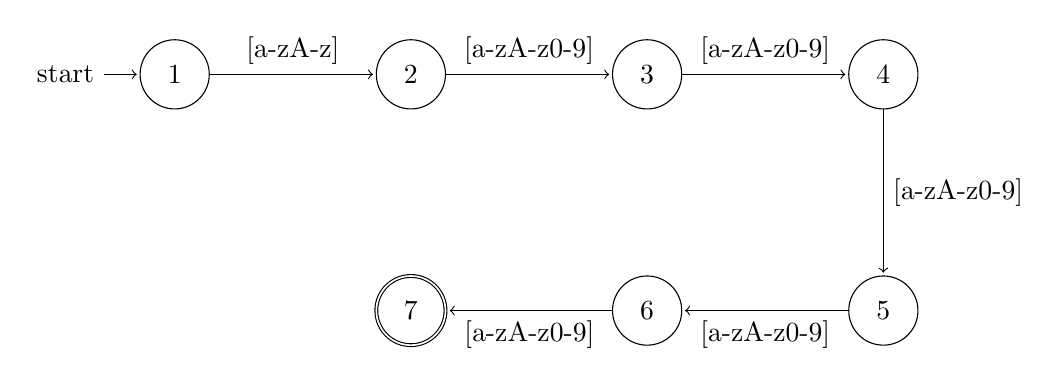
\begin{tikzpicture}[shorten >=1pt,node distance=3cm,auto]

  \node[initial,state]	(A)                    {$1$};
  \node[state]			(B) [right of=A] {$2$};
  \node[state]			(C) [right of=B] {$3$};
  \node[state]			(D) [right of=C] {$4$};
  \node[state]			(E) [below of=D]       {$5$};
  \node[state]	        (F) [left of=E]       {$6$};
  \node[state,accepting]	(G) [left of=F]       {$7$};

  \path [->]
        (A) edge              	node {[a-zA-z]} (B)
        (B) edge              	node {[a-zA-z0-9]} (C)
        (C) edge              	node {[a-zA-z0-9]} (D)
        (D) edge              	node {[a-zA-z0-9]} (E)
        (E) edge 				node {[a-zA-z0-9]} (F)
        (F) edge             	node {[a-zA-z0-9]} (G);
\end{tikzpicture} 
\end{figure}

\begin{figure}[H]
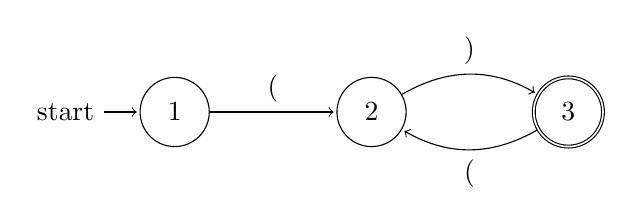
\begin{tikzpicture}[shorten >=1pt,node distance=2.5cm,auto]

  \node[initial,state]	(A)                    {$1$};
  \node[state]			(B) [right of=A] {$2$};
  \node[state, accepting]			(C) [right of=B] {$3$};

  \path [->]
        (A) edge              	node {(} (B)
        (B) edge  [bend left] 	node {)} (C)
        (C) edge  [bend left] 	node {(} (B);
\end{tikzpicture} 
\end{figure}
\section*{Exercise 6}
Regex:

\texttt{(")($\sum$|"")*(")}

\noindent FA:
\begin{figure}[H]
\begin{tikzpicture}[shorten >=1pt,node distance=2.5cm,auto]

  \node[initial,state]	    (A)                    {$1$};
  \node[state]			    (B) [right of=A] {$2$};
  \node[state, accepting]    (C) [right of=B] {$4$};
  \node[state]              (D) [above of=B] {$3$};

  \path [->]
        (A) edge                 node {"}         (B)
        (B) edge               	 node {"}         (C)
            edge  [bend left]    node {"}         (D)
            edge  [loop below]   node {$\sum$}    (B)
        (D) edge  [bend left]    node {"}         (B);
\end{tikzpicture} 
\end{figure}

\section*{Exercise 7.1}
(La+\textbackslash \ *)                            \\
(La+\textbackslash \ *)\{2\}                       \\
(La+\textbackslash \ *)\{3\}(Li\textbackslash \ *) \\

\section*{Exercise 7.2}
\begin{figure}[H]
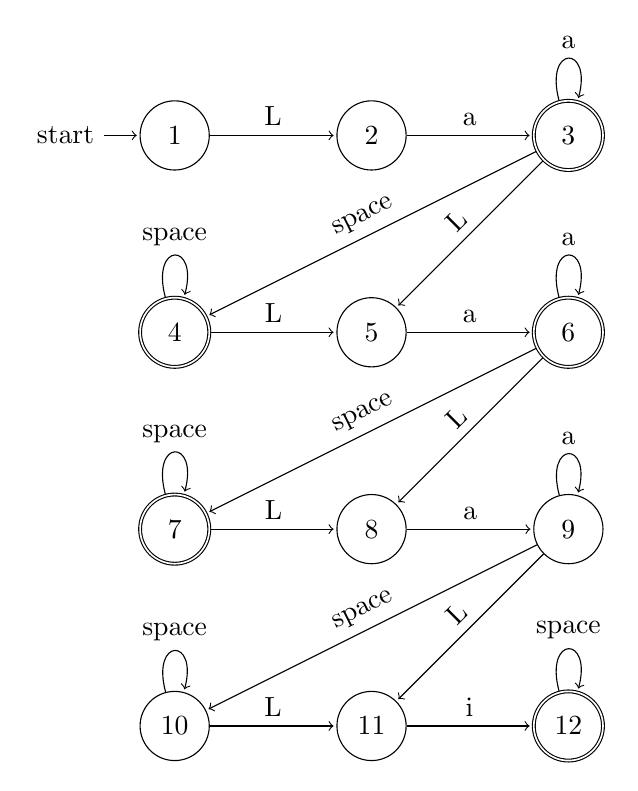
\begin{tikzpicture}[shorten >=1pt,node distance=2.5cm,auto]

  \node[initial,state]	    (A)              {$1$};
  \node[state]			    (B) [right of=A] {$2$};
  \node[state, accepting]   (C) [right of=B] {$3$};
  \node[state, accepting]   (D) [below of=A] {$4$};
  \node[state]			    (E) [right of=D]  {$5$};
  \node[state, accepting]   (F) [right of=E]  {$6$};
  \node[state, accepting]   (G) [below of=D] {$7$};
  \node[state]			    (H) [right of=G] {$8$};
  \node[state]              (I) [right of=H] {$9$};
  \node[state]              (J) [below of=G] {$10$};
  \node[state]			    (K) [right of=J]  {$11$};
  \node[state, accepting]   (L) [right of=K]  {$12$};

  \path [->]
        (A) edge               node                 {L}     (B)
        (B) edge               node                 {a}     (C)
        (C) edge  [loop above] node                 {a}     (C)
            edge               node [sloped, above] {space} (D)
            edge               node [sloped]        {L}     (E)
        (D) edge               node                 {L}     (E)
            edge  [loop above] node                 {space} (D)
        (E) edge               node                 {a}     (F)
        (F) edge  [loop above] node                 {a}     (F)
            edge               node [sloped, above] {space} (G)
            edge               node [sloped]        {L}     (H)
        (G) edge               node                 {L}     (H)
            edge  [loop above] node                 {space} (G)
        (H) edge               node                 {a}     (I)
        (I) edge  [loop above] node                 {a}     (I)
            edge               node [sloped, above] {space} (J)
            edge               node [sloped]        {L}     (K)
        (J) edge               node                 {L}     (K)
            edge  [loop above] node                 {space} (J)
        (K) edge               node                 {i}     (L)
        (L) edge  [loop above] node                 {space} (L);
\end{tikzpicture} 
\end{figure}

\section*{Exercise 7.3}
`Laaaa La' + `Laa'     \\
`La' + `La La La Li'

\section*{Exercise 15}
\begin{tabular}{l|p{11cm}} \hline

Sentential form
& A string is a sentential form if it occurs at a step in a valid derivation. \\\hline

Parse tree
& A graph representation of a derivation. \\\hline

Ambiguity
& Ambiguity occurs when a sentence in the language of a grammar derives in more than one derivation \\\hline

Left / right recursion
& Left recursion occurs if a non-terminal symbol can derive to a sentential form with itself as the leftmost symbol. Right recursion is the opposite. \\\hline

Recursive-descent parsing
& Parsing with a set of mutually recursive procedures. Each non-terminal has such a procedure. Simple and efficient for backtrack-free grammars. \\\hline

LL(x)
& A left-to-right leftmost parser with a lookahead of x. Reads the input from left to right and uses leftmost derivation to rewrite it. Parses it top-down with a lookahead of x. \\\hline

Bottom-up parsing
& Parsing from the leaves of a parse tree to the top / root. Creates a leaf node of the tree for a word returned by the scanner and works its way up with other (non)terminals to reach the top / root. \\\hline

LR(x)
& A left-to-right rightmost parser with a lookahead of x. Reads the input from left to right and uses rightmost derivation to rewrite it. Parses it top-down with a lookahead of x. \\\hline

\end{tabular}

\section*{Exercise 16.1}

\subsection*{Leftmost derivations}
\noindent Number 1

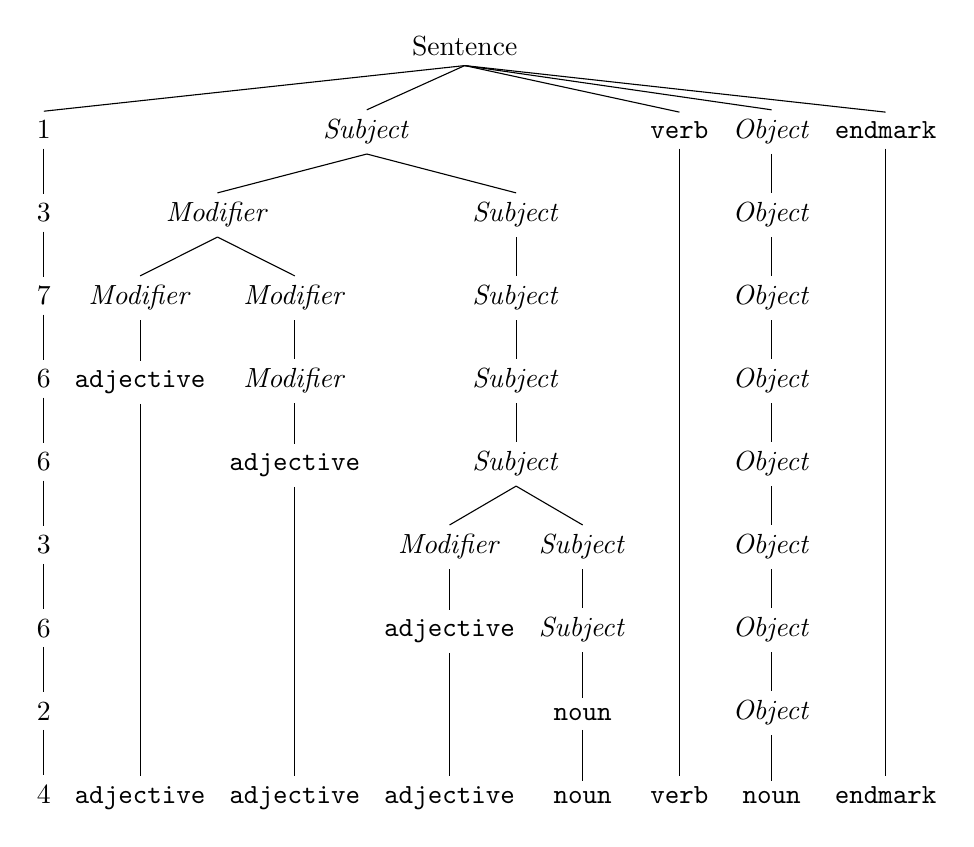
\begin{tikzpicture}

\tikzset{frontier/.style={distance from root=270pt}}

\Tree [.Sentence 
        [.1 [.3 [.7 [.6 [.6 [.3 [.6 [.2 4 ] ] ] ] ] ] ] ]
        [.\textit{Subject} 
            [.\textit{Modifier} 
                [.\textit{Modifier} 
                    [.\texttt{adjective} \texttt{adjective} ]
                ]
                [.\textit{Modifier} 
                    [.\textit{Modifier} 
                        [.\texttt{adjective} \texttt{adjective} ]
                    ]
                ]
            ]
            [.\textit{Subject} 
                [.\textit{Subject} 
                    [.\textit{Subject} 
                        [.\textit{Subject} 
                            [.\textit{Modifier} 
                                [.\texttt{adjective} \texttt{adjective} ]
                            ]
                            [.\textit{Subject} 
                                [.\textit{Subject} 
                                    [.\texttt{noun} \texttt{noun} ]    
                                ]
                            ]
                        ]
                    ]
                ]
            ]
        ]
        [.\texttt{verb} \texttt{verb} ]
        [.\textit{Object}
            [.\textit{Object}
                [.\textit{Object}
                    [.\textit{Object}
                        [.\textit{Object}
                            [.\textit{Object}
                                [.\textit{Object}
                                    [.\textit{Object}
                                        \texttt{noun}  
                                    ]  
                                ]
                            ]
                        ]
                    ]
                ]
            ]
        ]
        [.\texttt{endmark} \texttt{endmark} ]
    ]

\end{tikzpicture}

\noindent Number 2

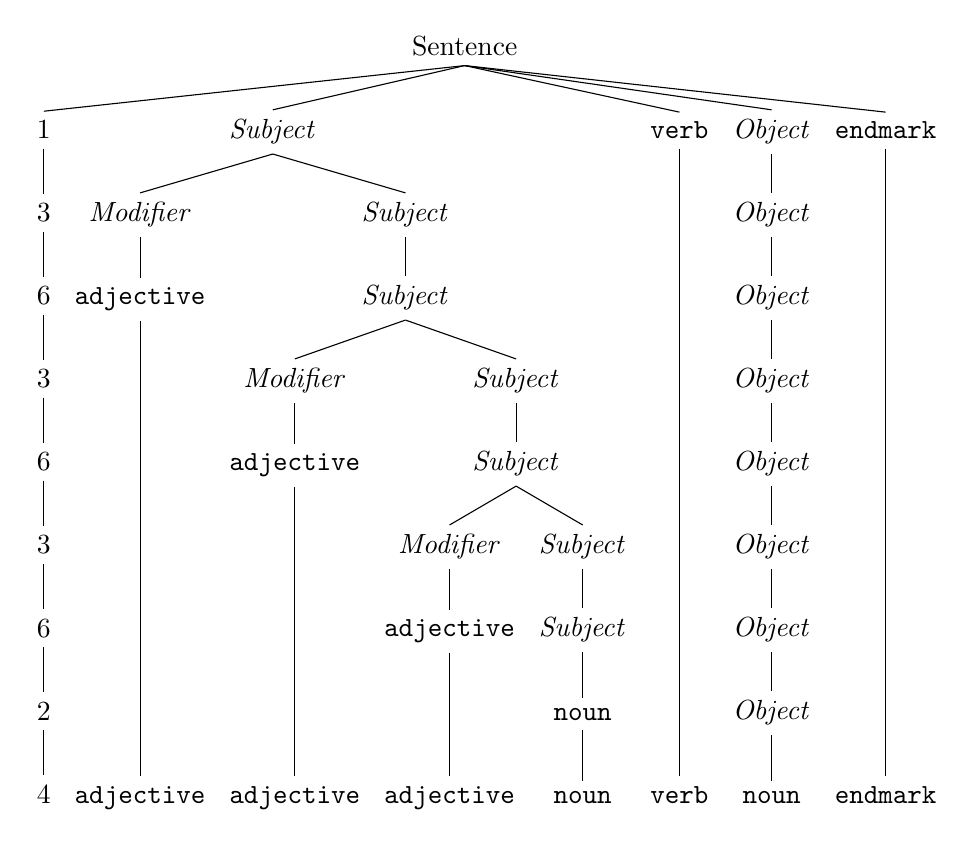
\begin{tikzpicture}

\tikzset{frontier/.style={distance from root=270pt}}

\Tree [.Sentence 
        [.1 [.3 [.6 [.3 [.6 [.3 [.6 [.2 4 ] ] ] ] ] ] ] ]
        [.\textit{Subject} 
            [.\textit{Modifier} 
                [.\texttt{adjective} \texttt{adjective} ]
            ]
            [.\textit{Subject} 
                [.\textit{Subject} 
                    [.\textit{Modifier} 
                        [.\texttt{adjective} \texttt{adjective} ]
                    ]
                    [.\textit{Subject} 
                        [.\textit{Subject} 
                            [.\textit{Modifier} 
                                [.\texttt{adjective} \texttt{adjective} ]
                            ]
                            [.\textit{Subject} 
                                [.\textit{Subject} 
                                    [.\texttt{noun} \texttt{noun} ]
                                ]
                            ]
                        ]
                    ]
                ]
            ]
        ]
        [.\texttt{verb} \texttt{verb} ]
        [.\textit{Object}
            [.\textit{Object}
                [.\textit{Object}
                    [.\textit{Object}
                        [.\textit{Object}
                            [.\textit{Object}
                                [.\textit{Object}
                                    [.\textit{Object}
                                        \texttt{noun}  
                                    ]  
                                ]
                            ]
                        ]
                    ]
                ]
            ]
        ]
        [.\texttt{endmark} \texttt{endmark} ]
    ]

\end{tikzpicture} 

\noindent Number 3

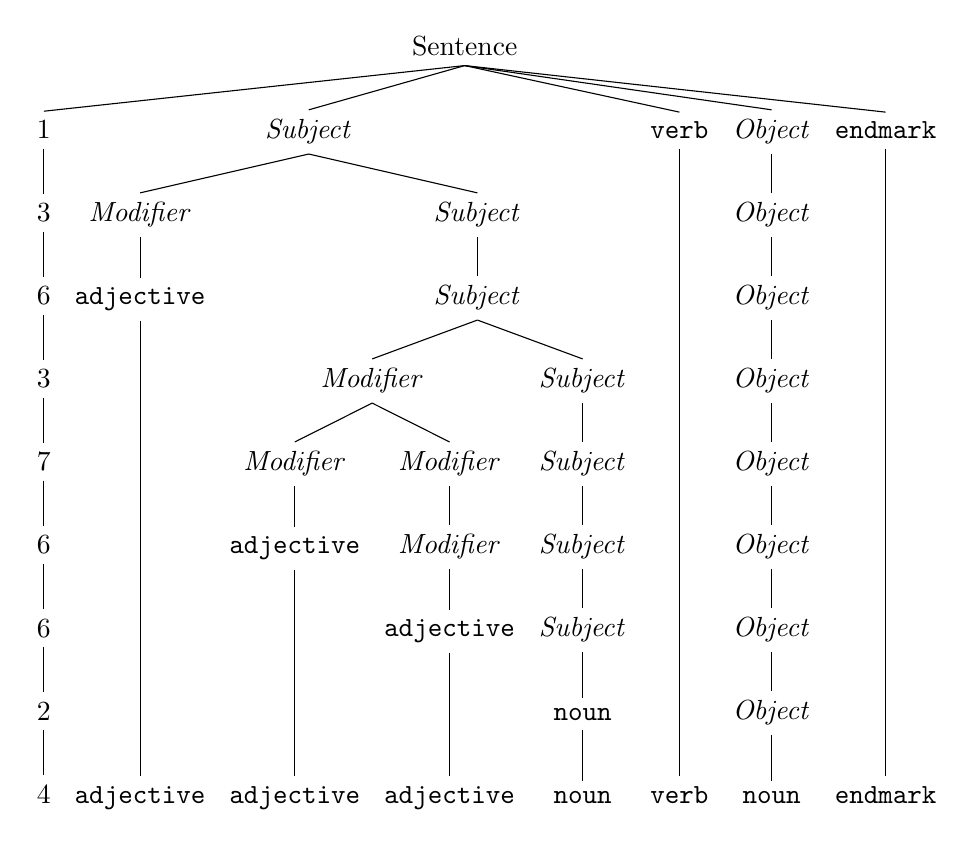
\begin{tikzpicture}

\tikzset{frontier/.style={distance from root=270pt}}

\Tree [.Sentence 
        [.1 [.3 [.6 [.3 [.7 [.6 [.6 [.2 4 ] ] ] ] ] ] ] ]
        [.\textit{Subject} 
            [.\textit{Modifier} 
                [.\texttt{adjective} \texttt{adjective} ]
            ]
            [.\textit{Subject} 
                [.\textit{Subject} 
                    [.\textit{Modifier} 
                        [.\textit{Modifier} 
                            [.\texttt{adjective} \texttt{adjective} ]
                        ]
                        [.\textit{Modifier} 
                            [.\textit{Modifier} 
                                [.\texttt{adjective} \texttt{adjective} ]
                            ]
                        ]
                    ]
                    [.\textit{Subject} 
                        [.\textit{Subject} 
                            [.\textit{Subject} 
                                [.\textit{Subject} 
                                    [.\texttt{noun} \texttt{noun} ]
                                ]
                            ]
                        ]
                    ]
                ]
            ]
        ]
        [.\texttt{verb} \texttt{verb} ]
        [.\textit{Object}
            [.\textit{Object}
                [.\textit{Object}
                    [.\textit{Object}
                        [.\textit{Object}
                            [.\textit{Object}
                                [.\textit{Object}
                                    [.\textit{Object}
                                        \texttt{noun}  
                                    ]  
                                ]
                            ]
                        ]
                    ]
                ]
            ]
        ]
        [.\texttt{endmark} \texttt{endmark} ]
    ]

\end{tikzpicture} 

\noindent Number 4

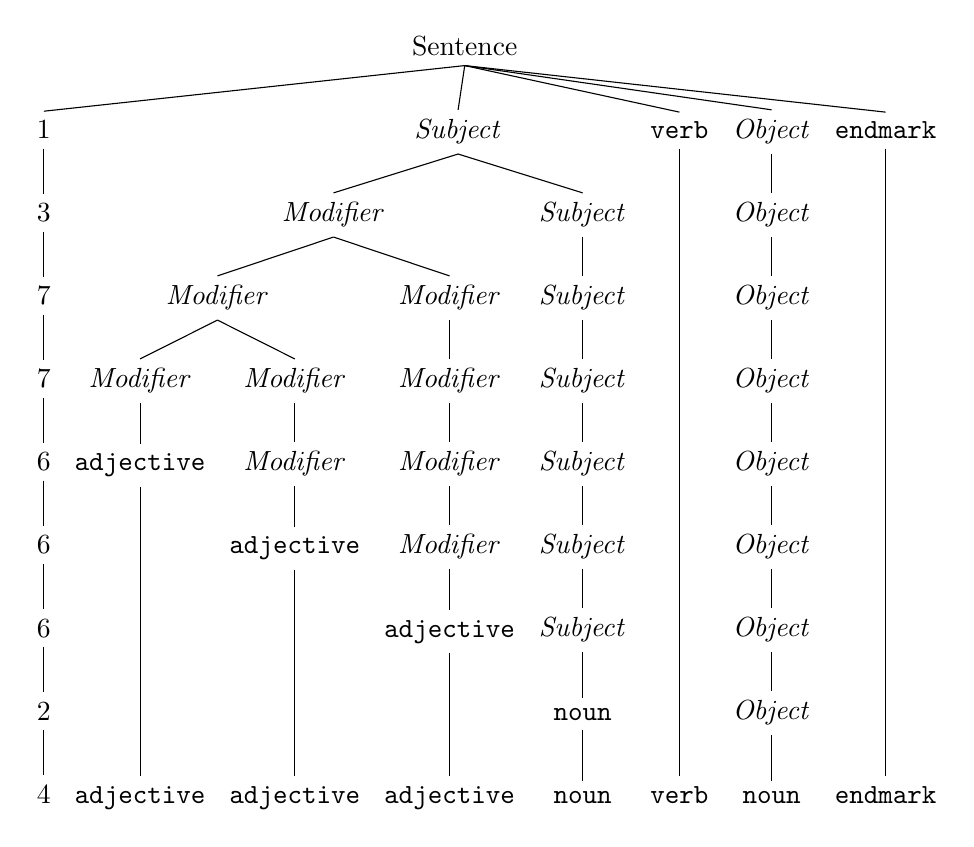
\begin{tikzpicture}

\tikzset{frontier/.style={distance from root=270pt}}

\Tree [.Sentence 
        [.1 [.3 [.7 [.7 [.6 [.6 [.6 [.2 4 ] ] ] ] ] ] ] ]
        [.\textit{Subject} 
            [.\textit{Modifier} 
                [.\textit{Modifier} 
                    [.\textit{Modifier} 
                        [.\texttt{adjective} \texttt{adjective} ]
                    ]
                    [.\textit{Modifier} 
                        [.\textit{Modifier} 
                            [.\texttt{adjective} \texttt{adjective} ]
                        ]
                    ]
                ]
                [.\textit{Modifier} 
                    [.\textit{Modifier} 
                        [.\textit{Modifier} 
                            [.\textit{Modifier} 
                                [.\texttt{adjective} \texttt{adjective} ]
                            ]
                        ]
                    ]
                ]
            ]
            [.\textit{Subject} 
                [.\textit{Subject}                     
                    [.\textit{Subject} 
                        [.\textit{Subject} 
                            [.\textit{Subject} 
                                [.\textit{Subject} 
                                    [.\texttt{noun} \texttt{noun} ]
                                ]
                            ]
                        ]
                    ]
                ]
            ]
        ]
        [.\texttt{verb} \texttt{verb} ]
        [.\textit{Object}
            [.\textit{Object}
                [.\textit{Object}
                    [.\textit{Object}
                        [.\textit{Object}
                            [.\textit{Object}
                                [.\textit{Object}
                                    [.\textit{Object}
                                        \texttt{noun}  
                                    ]  
                                ]
                            ]
                        ]
                    ]
                ]
            ]
        ]
        [.\texttt{endmark} \texttt{endmark} ]
    ]

\end{tikzpicture} 

\noindent Number 5

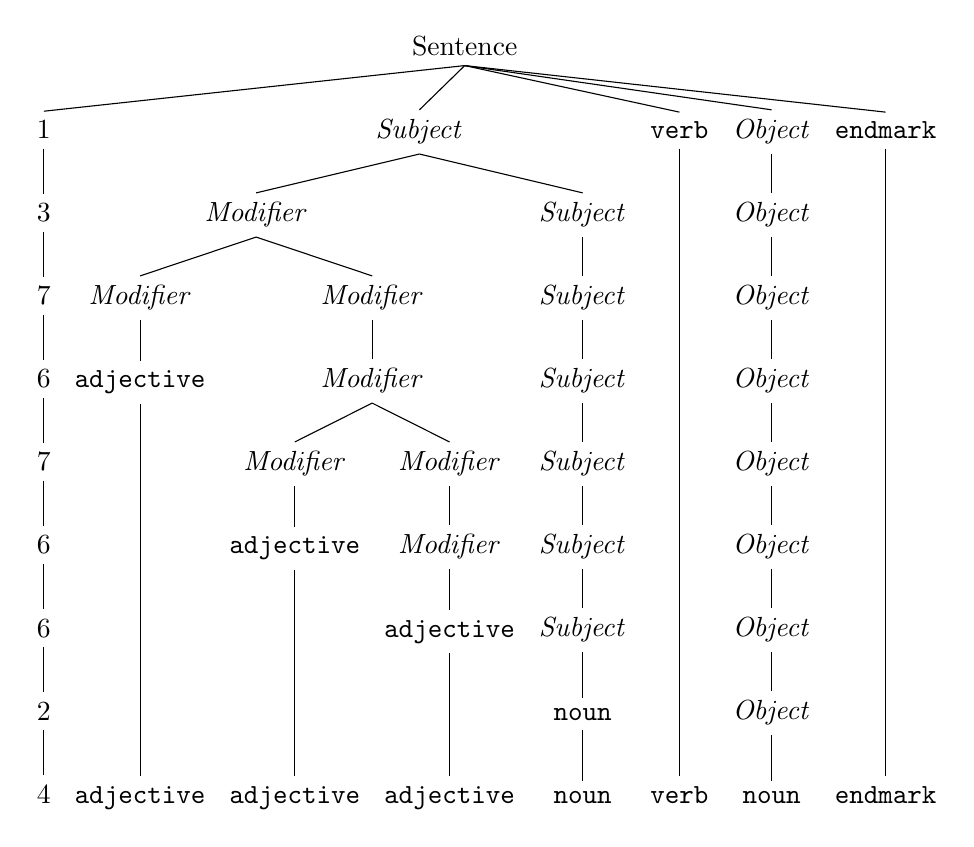
\begin{tikzpicture}

\tikzset{frontier/.style={distance from root=270pt}}

\Tree [.Sentence 
        [.1 [.3 [.7 [.6 [.7 [.6 [.6 [.2 4 ] ] ] ] ] ] ] ]
        [.\textit{Subject}
            [.\textit{Modifier} 
                [.\textit{Modifier} 
                    [.\texttt{adjective} \texttt{adjective} ]
                ]
                [.\textit{Modifier} 
                    [.\textit{Modifier} 
                        [.\textit{Modifier} 
                            [.\texttt{adjective} \texttt{adjective} ]
                        ]
                        [.\textit{Modifier} 
                            [.\textit{Modifier} 
                                [.\texttt{adjective} \texttt{adjective} ]
                            ]
                        ]
                    ]
                ]
            ]
            [.\textit{Subject} 
                [.\textit{Subject}                     
                    [.\textit{Subject} 
                        [.\textit{Subject} 
                            [.\textit{Subject} 
                                [.\textit{Subject} 
                                    [.\texttt{noun} \texttt{noun} ]
                                ]
                            ]
                        ]
                    ]
                ]
            ]
        ]
        [.\texttt{verb} \texttt{verb} ]
        [.\textit{Object}
            [.\textit{Object}
                [.\textit{Object}
                    [.\textit{Object}
                        [.\textit{Object}
                            [.\textit{Object}
                                [.\textit{Object}
                                    [.\textit{Object}
                                        \texttt{noun}  
                                    ]  
                                ]
                            ]
                        ]
                    ]
                ]
            ]
        ]
        [.\texttt{endmark} \texttt{endmark} ]
    ]
\end{tikzpicture} 

\subsection*{rightmost derivations}

\noindent Number 1

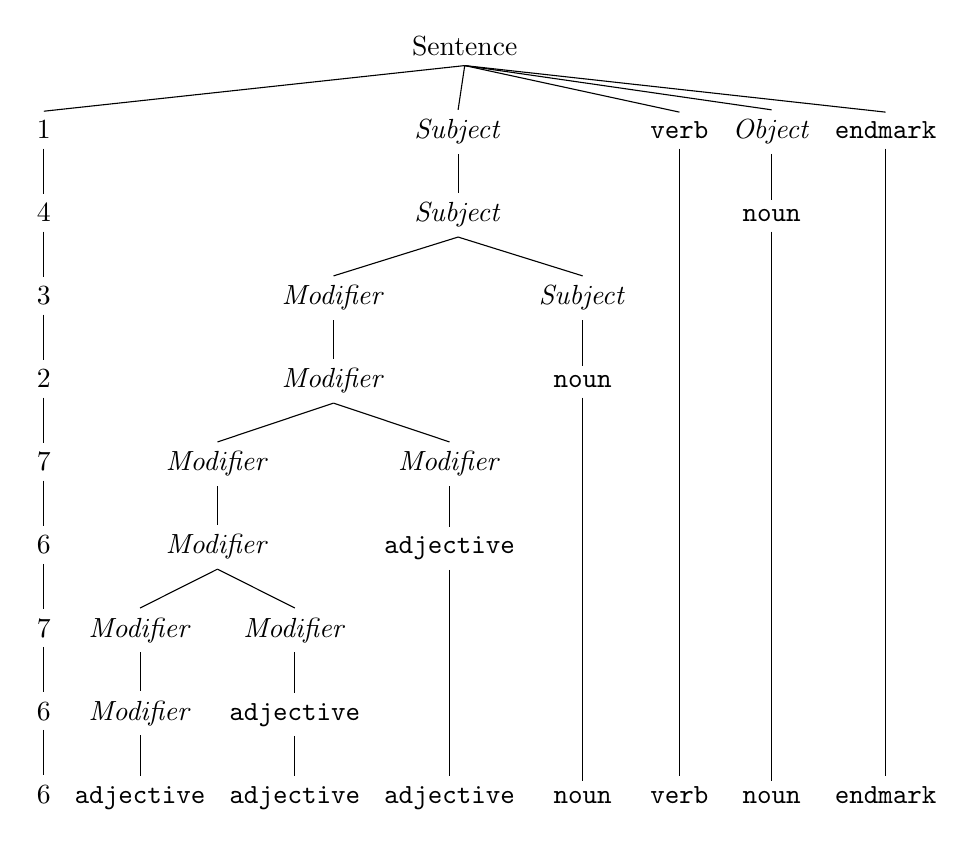
\begin{tikzpicture}

\tikzset{frontier/.style={distance from root=270pt}}

\Tree [.Sentence 
        [.1 [.4 [.3 [.2 [.7 [.6 [.7 [.6 6 ] ] ] ] ] ] ] ]
        [.\textit{Subject}
            [.\textit{Subject}
	            [.\textit{Modifier}
	                [.\textit{Modifier}
		                [.\textit{Modifier} 
		                    [.\textit{Modifier}
		                        [.\textit{Modifier} 
		                            [.\textit{Modifier} 
		                                \texttt{adjective}
		                            ]
		                        ] 
		                        [.\textit{Modifier} 
		                            [.\texttt{adjective} \texttt{adjective} ]
		                        ]
		                    ]
		                ]
		                [.\textit{Modifier} 
		                    [.\texttt{adjective} \texttt{adjective} ]
		                ]   
		            ] 
	            ]
	            [.\textit{Subject} 
	                [.\texttt{noun} \texttt{noun} ]
	            ]
	        ]
        ]
        [.\texttt{verb} \texttt{verb} ]
        [.\textit{Object}
            [.\texttt{noun} \texttt{noun} ]
        ]
        [.\texttt{endmark} \texttt{endmark} ]
    ]
\end{tikzpicture} 

\noindent Number 2

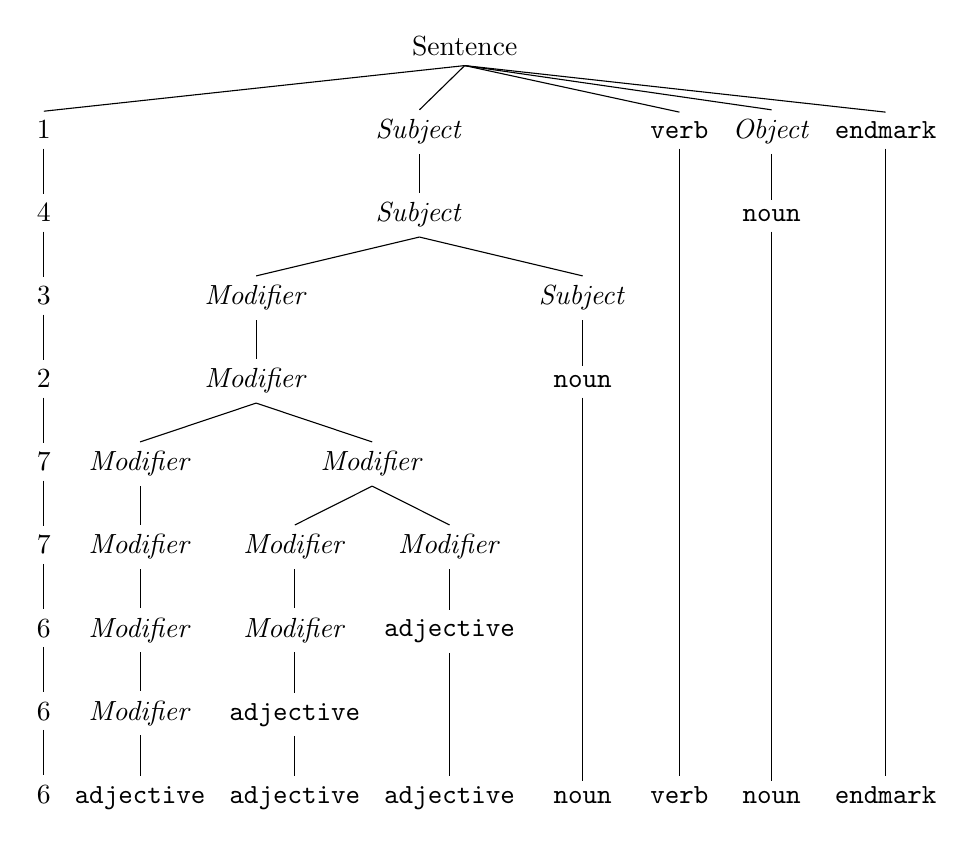
\begin{tikzpicture}

\tikzset{frontier/.style={distance from root=270pt}}

\Tree [.Sentence 
        [.1 [.4 [.3 [.2 [.7 [.7 [.6 [.6 6 ] ] ] ] ] ] ] ]
        [.\textit{Subject}
            [.\textit{Subject}
	            [.\textit{Modifier}
	                [.\textit{Modifier}
	                    [.\textit{Modifier} 
		                    [.\textit{Modifier} 
		                        [.\textit{Modifier} 
		                            [.\textit{Modifier} 
		                                \texttt{adjective}
		                            ]
		                        ]
		                    ]
		                ]
		                [.\textit{Modifier} 
	                        [.\textit{Modifier} 
	                            [.\textit{Modifier} 
	                                [.\texttt{adjective} \texttt{adjective} ]
	                            ]
	                        ]
	                        [.\textit{Modifier} 
	                            [.\texttt{adjective} \texttt{adjective} ]
	                        ]
		                ]
		            ] 
	            ]
	            [.\textit{Subject} 
	                [.\texttt{noun} \texttt{noun} ]
	            ]
	        ]
        ]
        [.\texttt{verb} \texttt{verb} ]
        [.\textit{Object}
            [.\texttt{noun} \texttt{noun} ]
        ]
        [.\texttt{endmark} \texttt{endmark} ]
    ]
\end{tikzpicture} 

\noindent Number 3

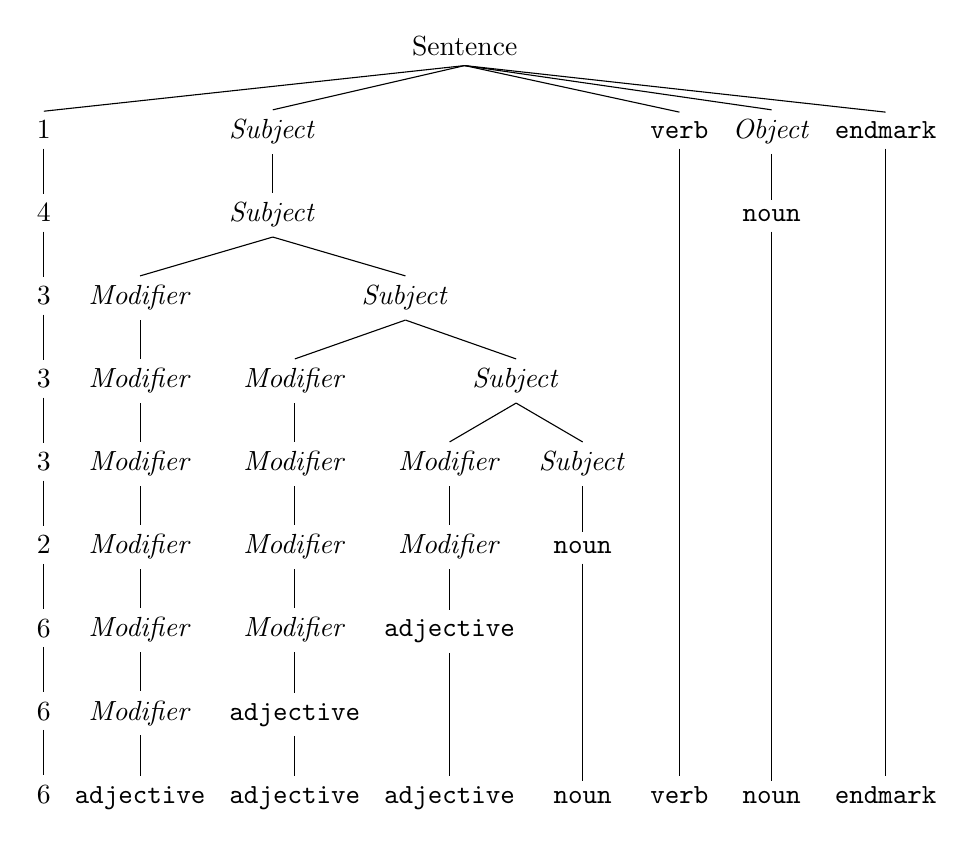
\begin{tikzpicture}

\tikzset{frontier/.style={distance from root=270pt}}

\Tree [.Sentence 
        [.1 [.4 [.3 [.3 [.3 [.2 [.6 [.6 6 ] ] ] ] ] ] ] ]
        [.\textit{Subject}
            [.\textit{Subject}
	            [.\textit{Modifier}
	                [.\textit{Modifier}
	                    [.\textit{Modifier} 
		                    [.\textit{Modifier} 
		                        [.\textit{Modifier} 
		                            [.\textit{Modifier} 
		                                \texttt{adjective}
		                            ]
		                        ]
		                    ]
		                ]
		            ] 
	            ]
	            [.\textit{Subject} 
	                [.\textit{Modifier}
	                    [.\textit{Modifier}
	                        [.\textit{Modifier}
                                [.\textit{Modifier}
                                    [.\texttt{adjective} \texttt{adjective} ]
                                ]
	                        ]
	                    ]
	                ]
	                [.\textit{Subject} 
		                [.\textit{Modifier}
	                        [.\textit{Modifier}
	                            [.\texttt{adjective} \texttt{adjective} ]
	                        ]
	                    ]
	                    [.\textit{Subject} 
		                    [.\texttt{noun} \texttt{noun} ]
	                    ]
	                ]
	            ]
	        ]
        ]
        [.\texttt{verb} \texttt{verb} ]
        [.\textit{Object}
            [.\texttt{noun} \texttt{noun} ]
        ]
        [.\texttt{endmark} \texttt{endmark} ]
    ]
\end{tikzpicture} 

\noindent Number 4

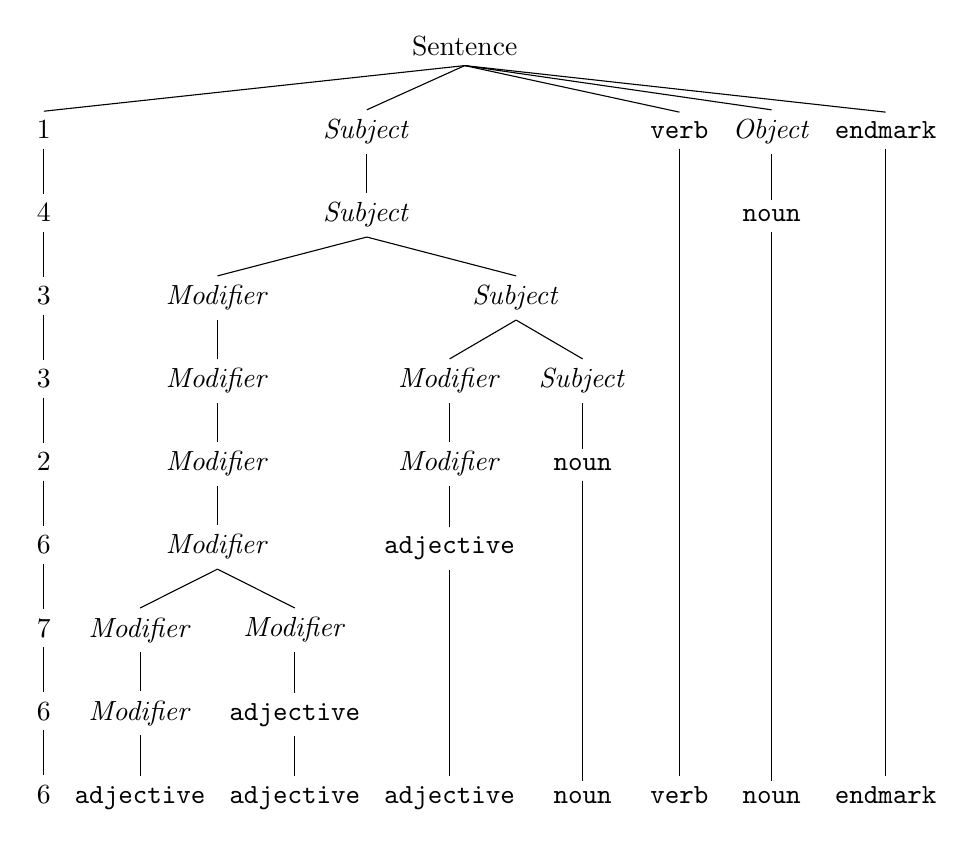
\begin{tikzpicture}

\tikzset{frontier/.style={distance from root=270pt}}

\Tree [.Sentence 
        [.1 [.4 [.3 [.3 [.2 [.6 [.7 [.6 6 ] ] ] ] ] ] ] ]
        [.\textit{Subject}
            [.\textit{Subject}
	            [.\textit{Modifier}
	                [.\textit{Modifier}
	                    [.\textit{Modifier} 
		                    [.\textit{Modifier}
		                        [.\textit{Modifier}
	                                [.\textit{Modifier}
	                                    \texttt{adjective}
	                                ]
		                        ]
		                        [.\textit{Modifier}
		                            [.\texttt{adjective} \texttt{adjective} ]
		                        ]
		                    ]
		                ]
		            ] 
	            ]
	            [.\textit{Subject} 
	                [.\textit{Modifier}
	                    [.\textit{Modifier}
	                        [.\texttt{adjective} \texttt{adjective} ]
	                    ]
	                ]
	                [.\textit{Subject} 
		                [.\texttt{noun} \texttt{noun} ]
	                ]
	            ]
	        ]
        ]
        [.\texttt{verb} \texttt{verb} ]
        [.\textit{Object}
            [.\texttt{noun} \texttt{noun} ]
        ]
        [.\texttt{endmark} \texttt{endmark} ]
    ]
\end{tikzpicture}

\noindent Number 4

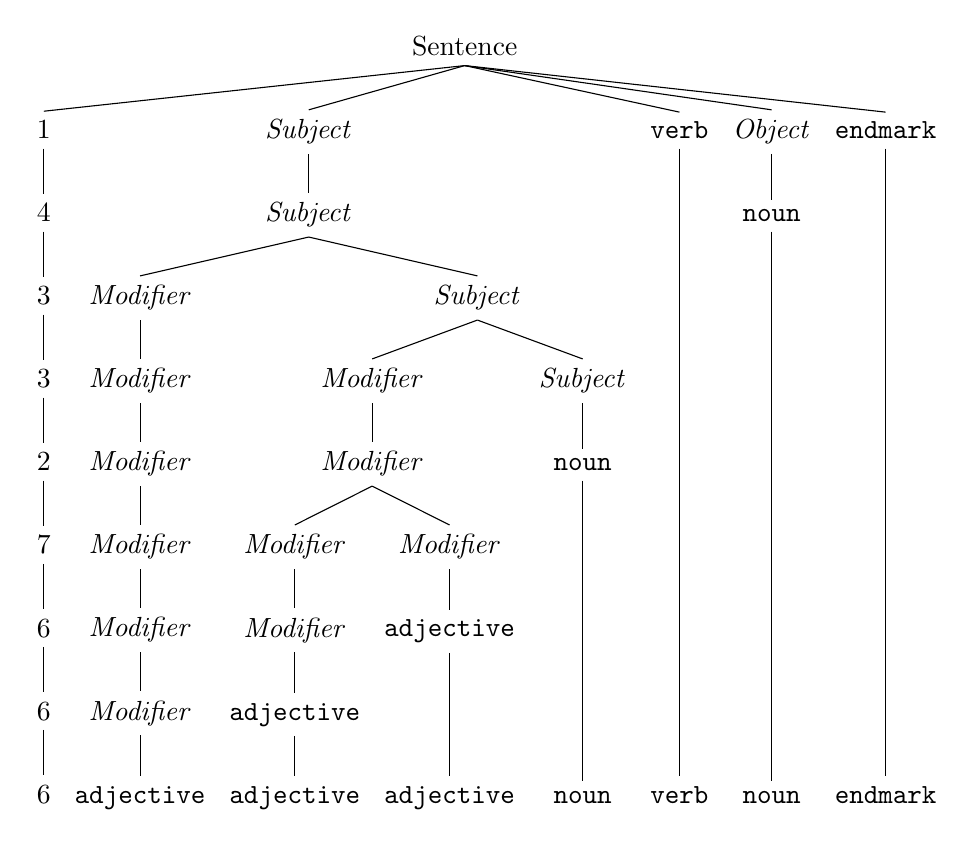
\begin{tikzpicture}

\tikzset{frontier/.style={distance from root=270pt}}

\Tree [.Sentence 
        [.1 [.4 [.3 [.3 [.2 [.7 [.6 [.6 6 ] ] ] ] ] ] ] ]
        [.\textit{Subject}
            [.\textit{Subject}
	            [.\textit{Modifier}
	                [.\textit{Modifier}
	                    [.\textit{Modifier} 
		                    [.\textit{Modifier}
		                        [.\textit{Modifier}
	                                [.\textit{Modifier}
	                                    \texttt{adjective}
	                                ]
		                        ]
		                    ]
		                ]
		            ] 
	            ]
	            [.\textit{Subject} 
	                [.\textit{Modifier}
	                    [.\textit{Modifier}
		                    [.\textit{Modifier}
		                        [.\textit{Modifier}
		                            [.\texttt{adjective} \texttt{adjective} ]
		                        ]
		                    ]
	                        [.\textit{Modifier}
	                            [.\texttt{adjective} \texttt{adjective} ]
	                        ]
	                    ]
	                ]
	                [.\textit{Subject} 
		                [.\texttt{noun} \texttt{noun} ]
	                ]
	            ]
	        ]
        ]
        [.\texttt{verb} \texttt{verb} ]
        [.\textit{Object}
            [.\texttt{noun} \texttt{noun} ]
        ]
        [.\texttt{endmark} \texttt{endmark} ]
    ]
\end{tikzpicture}

\section*{Exercise 16.2}
Rightmost derivation is the most clean one and does reflect the structure of the sentence in the best way, because of the continuous derivation of the subject. However, leftmost derivation

\section*{Exercise 16.3}
\begin{tabular}{llcl}
1
& \textbf{Sentence}
& $\rightarrow$
& \textbf{Subject} verb \textbf{Object} endmark	\\

2
& \textbf{Subject}
& $\rightarrow$
& noun \\

3
& \textbf{Subject}
& $\rightarrow$
& \textbf{Modifier' Subject} \\

4
& \textbf{Object}
& $\rightarrow$
& noun \\

5
& \textbf{Object}
& $\rightarrow$
& \textbf{Modifier' Object} \\

6
& \textbf{Modifier}
& $\rightarrow$
& adjective \\

7
& \textbf{Modifier'}
& $\rightarrow$
& \textbf{Modifier Modifier'} \\

\end{tabular}

\section*{Exercise 17}
Calculation of the FIRST set of all Terminals:\\

\begin{tabular}{|c|c|c|c|c|c|c|} \hline 
\textbf{assign}
& \textbf{if}
& \textbf{else}
& \textbf{then}
& \textbf{expr}
& \textbf{$\epsilon$}
& \textbf{eof} \\\hline 

assign
& if
& else
& then
& expr
& $\epsilon$
& eof \\\hline 
\end{tabular} \\

\noindent Calculation of the FIRST set of all Non-Terminals:\\

\begin{tabular}{|p{2cm}|c|} \hline 
\textbf{Stat}
& \textbf{ElsePart} \\\hline 

& \\\hline 
\end{tabular} \\

\begin{tabular}{|p{2cm}|c|} \hline 
\textbf{Stat}
& \textbf{ElsePart} \\\hline 

assign
& \\\hline 
\end{tabular} \\

\begin{tabular}{|p{2cm}|c|} \hline 
\textbf{Stat}
& \textbf{ElsePart} \\\hline 

assign, if
& else \\\hline 
\end{tabular} \\

\begin{tabular}{|p{2cm}|c|} \hline 
\textbf{Stat}
& \textbf{ElsePart} \\\hline

assign, if
& else, $\epsilon$ \\\hline 
\end{tabular}\\

\noindent Calculation of the FOLLOW set:\\

\begin{tabular}{|p{2cm}|c|} \hline 
\textbf{Stat}
& \textbf{ElsePart} \\\hline 

& \\\hline 
\end{tabular} \\

\begin{tabular}{|p{2cm}|c|} \hline 
\textbf{Stat}
& \textbf{ElsePart} \\\hline

eof
& \\\hline 
\end{tabular} \\

\begin{tabular}{|p{2cm}|c|} \hline 
\textbf{Stat}
& \textbf{ElsePart} \\\hline

eof
& eof \\\hline 
\end{tabular} \\

\begin{tabular}{|p{2cm}|c|} \hline 
\textbf{Stat}
& \textbf{ElsePart} \\\hline 

eof, else
& eof, else \\\hline 
\end{tabular}\\

\noindent Calculation of the FIRST+ set (only rule 4 is necessary):\\

\begin{tabular}{|c|c|c|c|} \hline 
& Production
& FIRST Set
& FIRST+ Set \\\hline

4
& \textbf{ElsePart} $\rightarrow \epsilon$
& \{$\epsilon$\}
& \{$\epsilon$, eof, else\} \\\hline 
\end{tabular}\\

\noindent The FIRST+ set of \textbf{ElsePart} $\rightarrow \epsilon$ (\{$\epsilon$, eof, else\}) is not disjoint with FIRST+ set of \textbf{ElsePart} $\rightarrow$ else Stat (\{else, $\epsilon$\}). Therefore, the grammar does not meet the criteria for \textit{LL(1)}\\

\section*{Exercise 18}
\begin{tabular}{llcl}
1
& \textbf{L}
& $\rightarrow$
& \textbf{R}a \\

2
& 
& $\vert$
& \textbf{Q}ba \\

3
& \textbf{R}
& $\rightarrow$
& aba \\

4
& 
& $\vert$
& caba \\

5
& 
& $\vert$
& \textbf{R}bc \\

6
& \textbf{Q}
& $\rightarrow$
& bbc \\

7
& 
& $\vert$
& bc \\
\end{tabular}\\

\noindent FIRST of Terminals: \\

\begin{tabular}{|c|c|c|c|c|} \hline 
\textbf{a}
& \textbf{b}
& \textbf{c}
& \textbf{eof}
& \textbf{$\epsilon$}\\\hline 

a
& b
& c
& eof
& $\epsilon$\\\hline  
\end{tabular} \\

\noindent FIRST of Non-Terminals: \\

\begin{tabular}{|c|c|c|} \hline 
\textbf{L}
& \textbf{R}
& \textbf{Q} \\\hline 

a, b, c
& a, c
& b \\\hline  
\end{tabular} \\

\noindent FOLLOW: \\

\begin{tabular}{|c|c|c|} \hline 
\textbf{L}
& \textbf{R}
& \textbf{Q} \\\hline 

eof
& eof, a, b, c
& eof, a, b \\\hline  
\end{tabular} \\

\noindent Problem: left recursion at rule 5 and double b at rules 6 and 7!  \\

\begin{tabular}{llcl}
1
& \textbf{L}
& $\rightarrow$
& \textbf{R}a \\

2
& 
& $\vert$
& \textbf{Q}ba \\

3
& \textbf{R}
& $\rightarrow$
& aba\textbf{R'} \\

4
& 
& $\vert$
& caba\textbf{R'} \\

6
& \textbf{Q}
& $\rightarrow$
& b\textbf{Q'} \\

8
& \textbf{R'}
& $\rightarrow$
& bc\textbf{R'} \\

9
& 
& $\vert$
& $\epsilon$ \\

10
& \textbf{Q'}
& $\rightarrow$
& bc \\

11
& 
& $\vert$
& c \\
\end{tabular} \\

\noindent Showing that the new grammar satisfies the \textit{LL(1)} condition: \\

\noindent FIRST of Terminals: \\

\begin{tabular}{|c|c|c|c|c|} \hline 
\textbf{a}
& \textbf{b}
& \textbf{c}
& \textbf{eof}
& \textbf{$\epsilon$}\\\hline 

a
& b
& c
& eof
& $\epsilon$\\\hline  
\end{tabular} \\

\noindent FIRST of Non-Terminals: \\

\begin{tabular}{|c|c|c|c|c|} \hline 
\textbf{L}
& \textbf{R}
& \textbf{Q}
& \textbf{R'}
& \textbf{Q'} \\\hline 

a, b, c
& a, c
& b
& b, $\epsilon$
& b, c \\\hline  
\end{tabular} \\

\noindent FOLLOW: \\

\begin{tabular}{|c|c|c|c|c|} \hline 
\textbf{L}
& \textbf{R}
& \textbf{Q}
& \textbf{R'}
& \textbf{Q'} \\\hline

eof
& a
& b
& a
& b \\\hline  
\end{tabular} \\

\noindent $\epsilon$ in rule 9, FIRST+ set: \\

\begin{tabular}{|c|c|c|c|} \hline 
& Production
& FIRST Set
& FIRST+ Set \\\hline

9
& \textbf{R'} $\rightarrow \epsilon$
& \{$\epsilon$\}
& \{$\epsilon$, a\} \\\hline 
\end{tabular}\\

\noindent Every FIRST+ set of every Non-Terminal rule-combination is disjoint, so this satisfies the \textit{LL(1)} condition!\\

\end{document}
